
\chapter{Design}

After analyzing the task and collecting the requirements, this chapter will go through the design of initial paper prototypes as well as higher fidelity software prototypes. I will also describe the architecture of the mobile application which is crucial for successful development, future extensions and maintenance. I will talk about different components that the application is composed of and how they cooperate to achieve desired functionality. This chapter contains several UML diagrams, all of which are simplified.

\section{Application Structure}

The application requirements give a thorough description of the features the app will offer. Upon the requirements I have designed the application navigation structure that I'd like to follow. Figure \ref{fig:structure} shows the hierarchy of the app's screens with somewhat simplified screen transitions. The root of the navigation is the Project List screen which will show lists of projects. For each project, the hierarchy then goes deeper to allow user to view further project information and to work with jobs, translation memories and term bases. Another application entry point is the screen for adding a job from an external application (e.g. from Mail or from a filesystem browser application).

\begin{figure}[]
	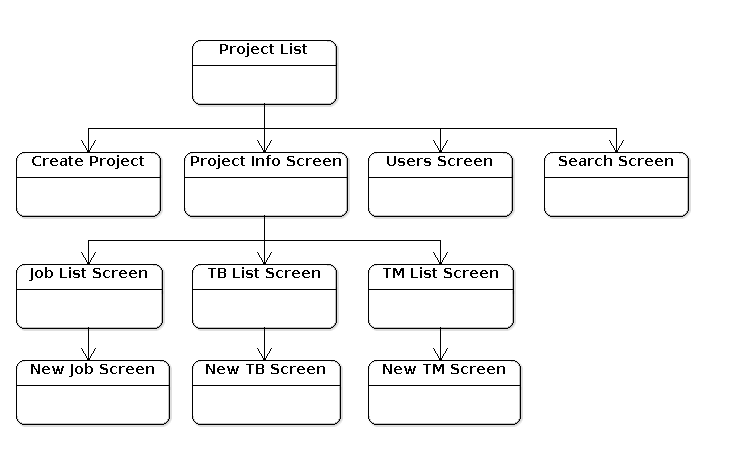
\includegraphics[width=1\textwidth]{argoUml/structure}
	\caption{Structure of the app's screens.}
	\label{fig:structure}
\end{figure}

\section{Prototyping}

Based on the collected requirements, a set of mockups was constructed. Some of these were later used to construct a prototype for an Android device that was used for tests with users. Both the mockups and the prototype consider the project manager role because its feature set is a superset of the one of the linguist role.

The mockups were discussed with employees of Memsource support team. Different ideas of presenting information to the user were brought up and consulted. Memsource support members provided feedback and deeper insight on how different features are used and whether they are needed. Understanding the workflow was important to designing the final mockups.

In the end, the prototype largely follows the structure of Memsource cloud, but it is simpler in terms of the number of supported options and gives off Android platform feel. The following pages contain several figures that present selected mockup screens.



\begin{figure}[]
	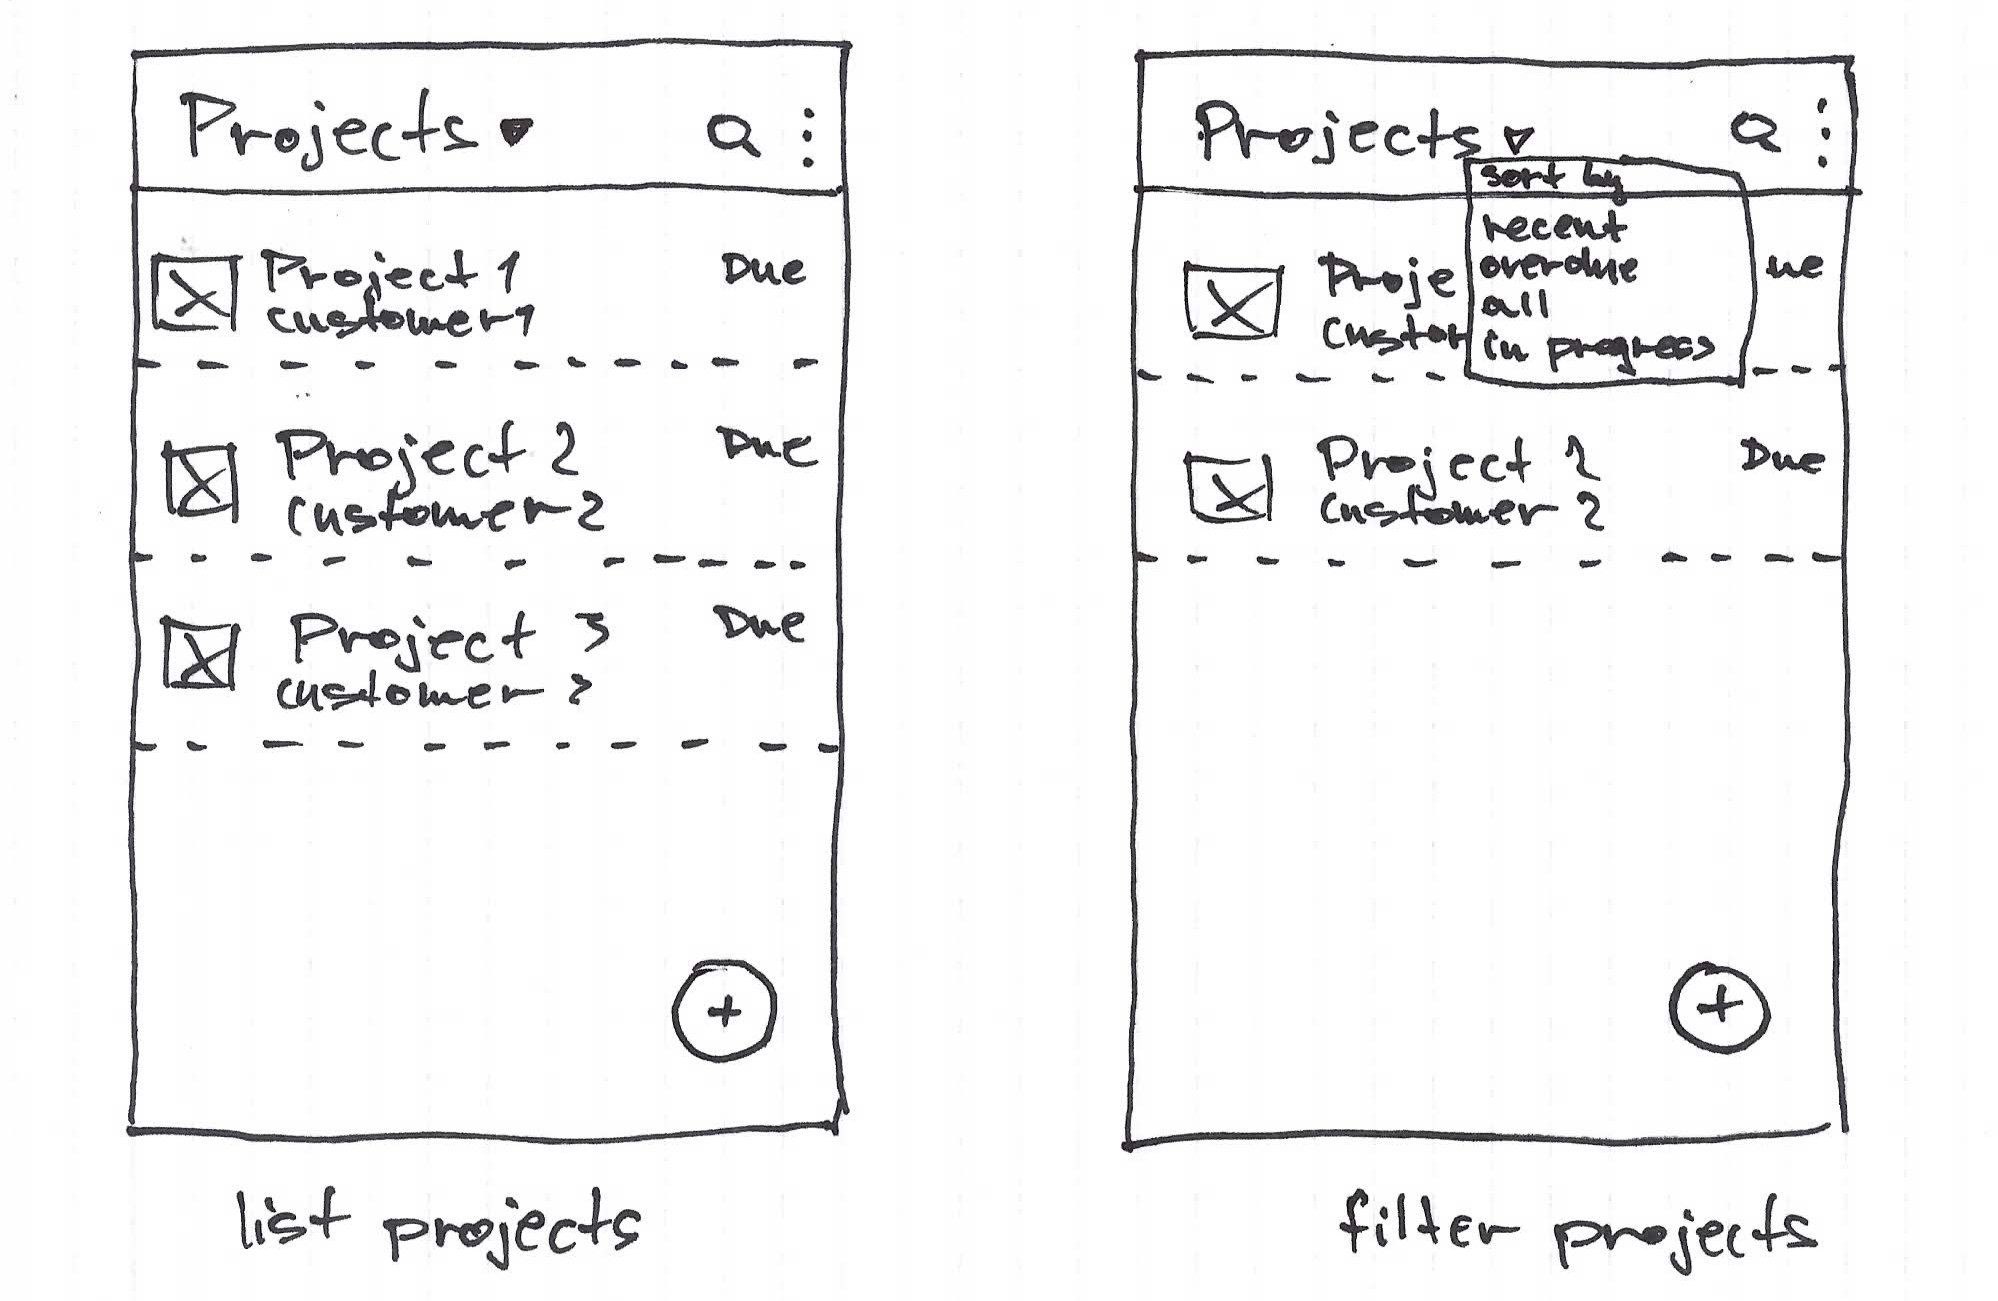
\includegraphics[width=0.7\textwidth]{pics/projects1}
	\caption{Mockups showing the project list screens. Second screen shows the chevron active, where user can filter displayed projects.}
	\label{mock2}
\end{figure}

\begin{figure}[H]
	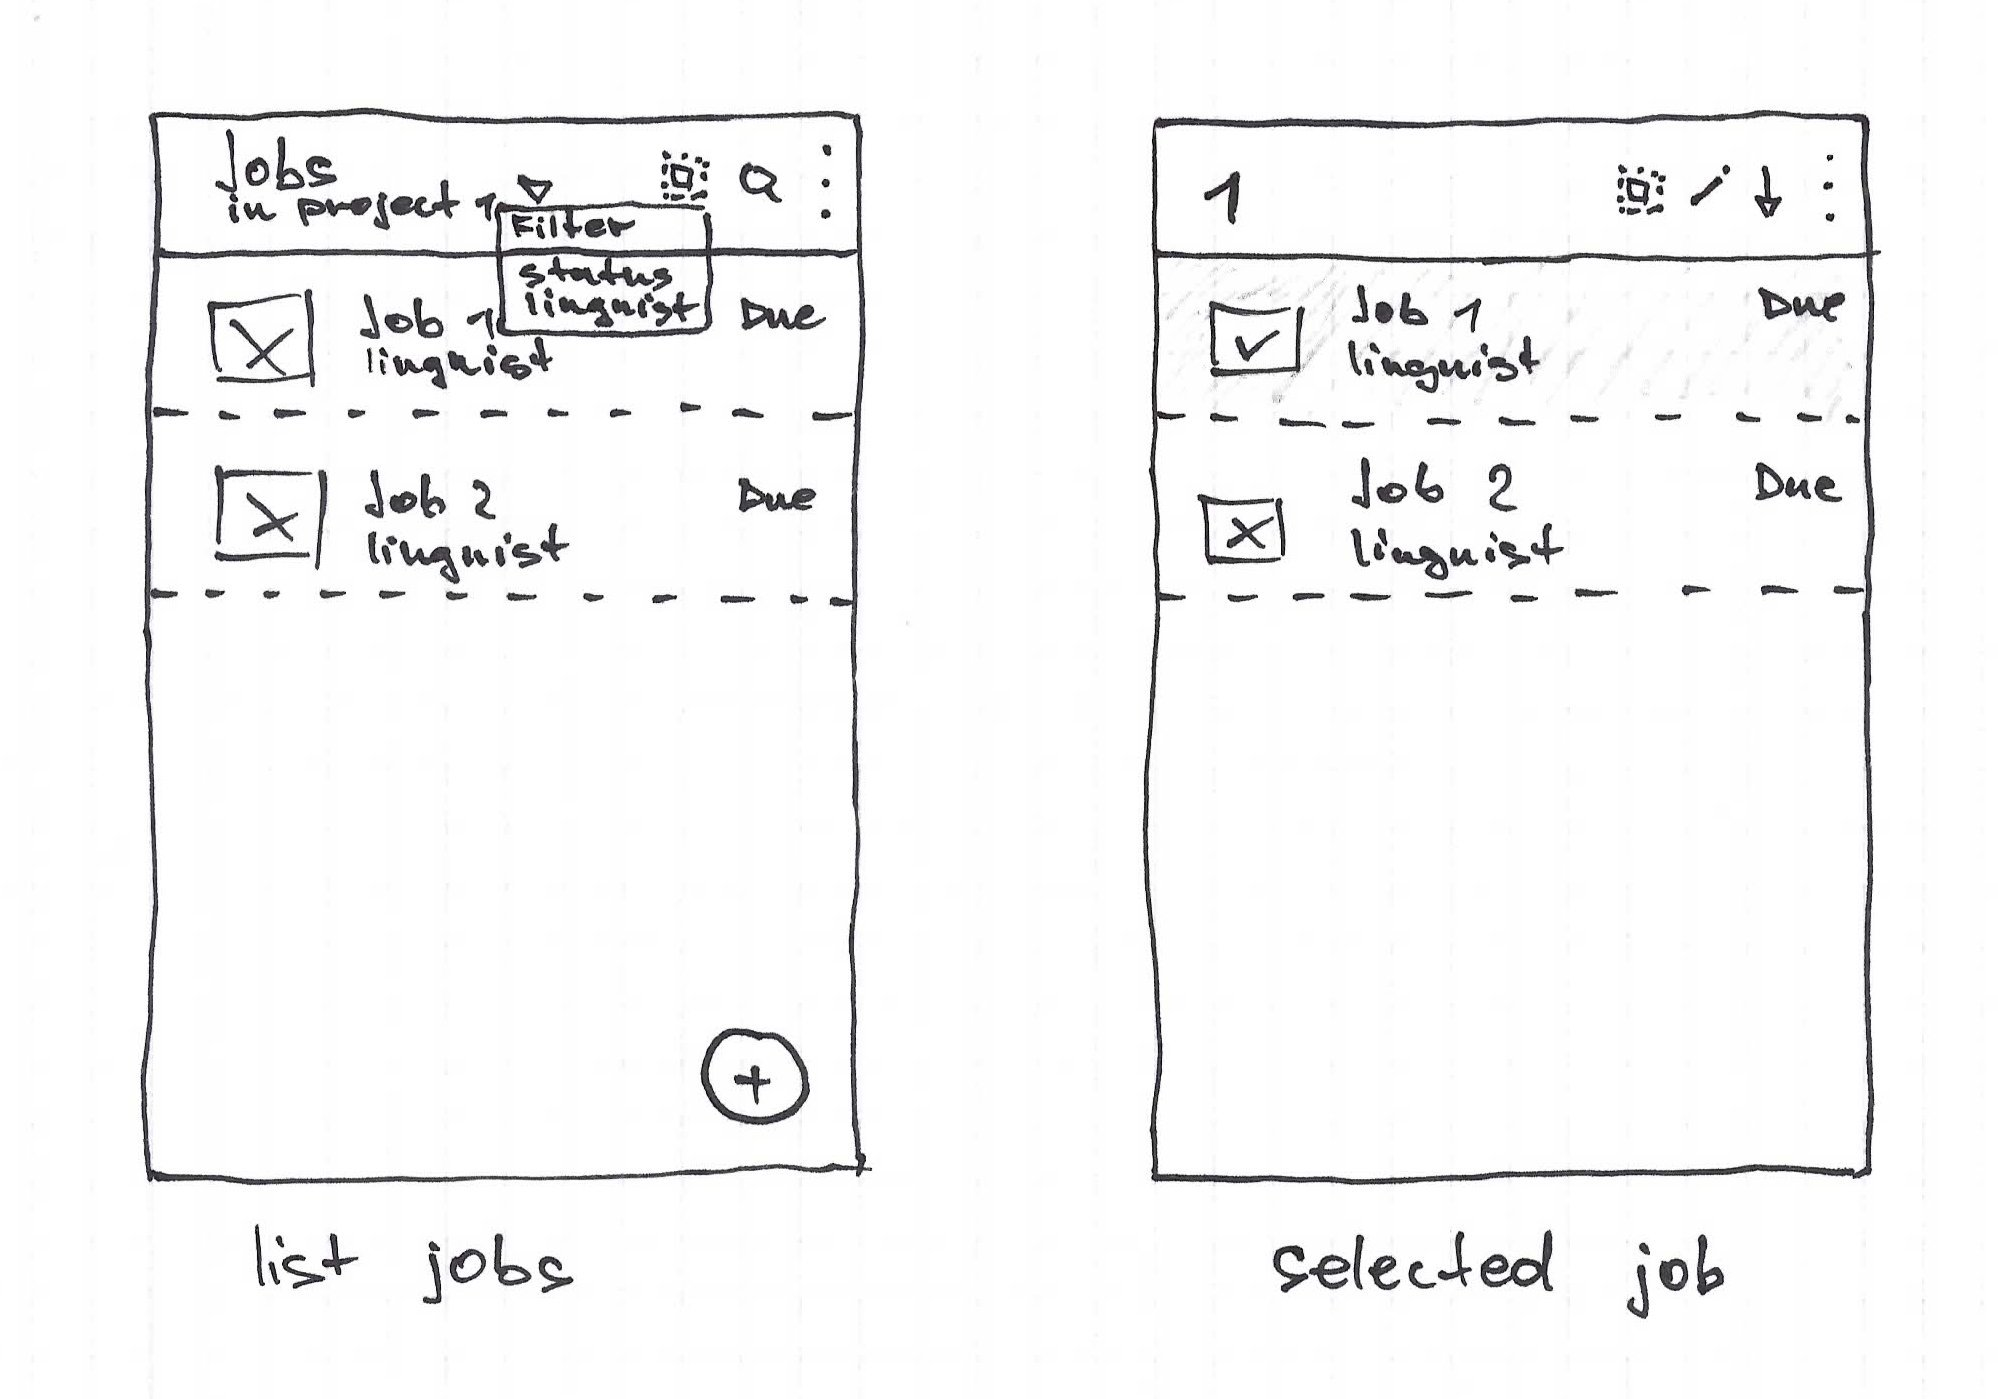
\includegraphics[width=0.7\textwidth]{pics/jobs1}
	\caption{Job list (left) and a mockup where ``Job 1'' is selected and different actions are available for it (right).}
	\label{mock3}
\end{figure}

\begin{figure}[H]
	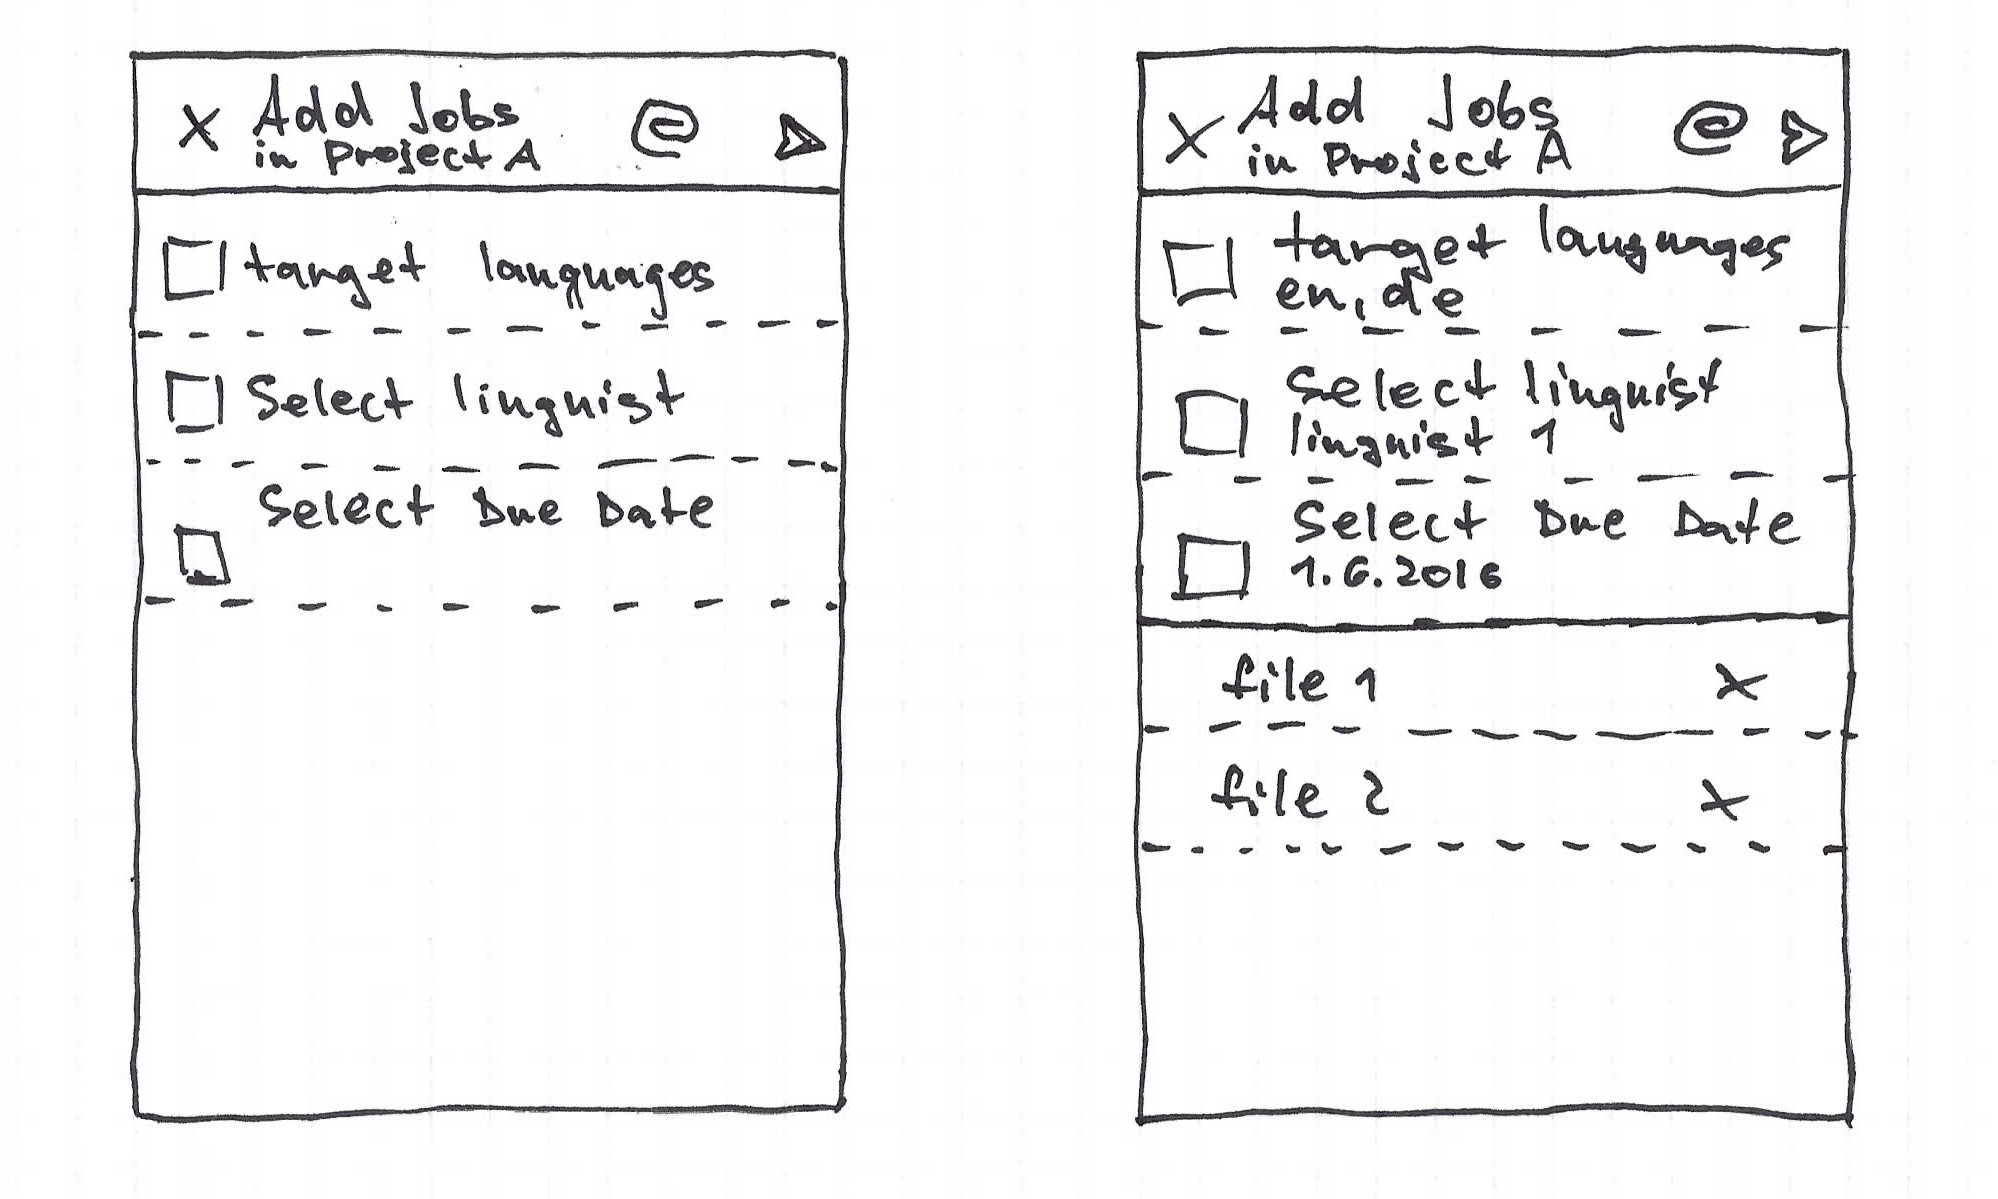
\includegraphics[width=0.7\textwidth]{pics/addJobs}
	\caption{Adding a new job to a project.}
	\label{mock4}
\end{figure}


Figure \ref{mock2} shows design of the project listing. There are controls for creating a project, searching, filtering (using the chevron) and getting the important information about user's projects. In figure \ref{fig:proto} you can see how filtering the projects changed in the final prototype. 

Figure \ref{mock3} shows a mockup of an opened project with translation jobs listed (first screen). The second screen shows a job being selected and the consequent changes in the navbar: the user can choose to edit, select all or download job. 

Figure \ref{mock4} contains the screens for adding a new job to a project from within the application. The figure shows two states of the same screen, first screen is waiting for user to enter needed information, the second displays the state when the information is entered, along with two files chosen for upload. In the prototype, the layout of these screens was preserved, except for division into two tabs: one for uploaded files and second for import settings.



For iOS, which has different interaction patters compared to Android, I created separate mockups of what the UI could look like. The figure (\ref{mock5}) shows the mockup of job listing and handling.

\begin{figure}[]
	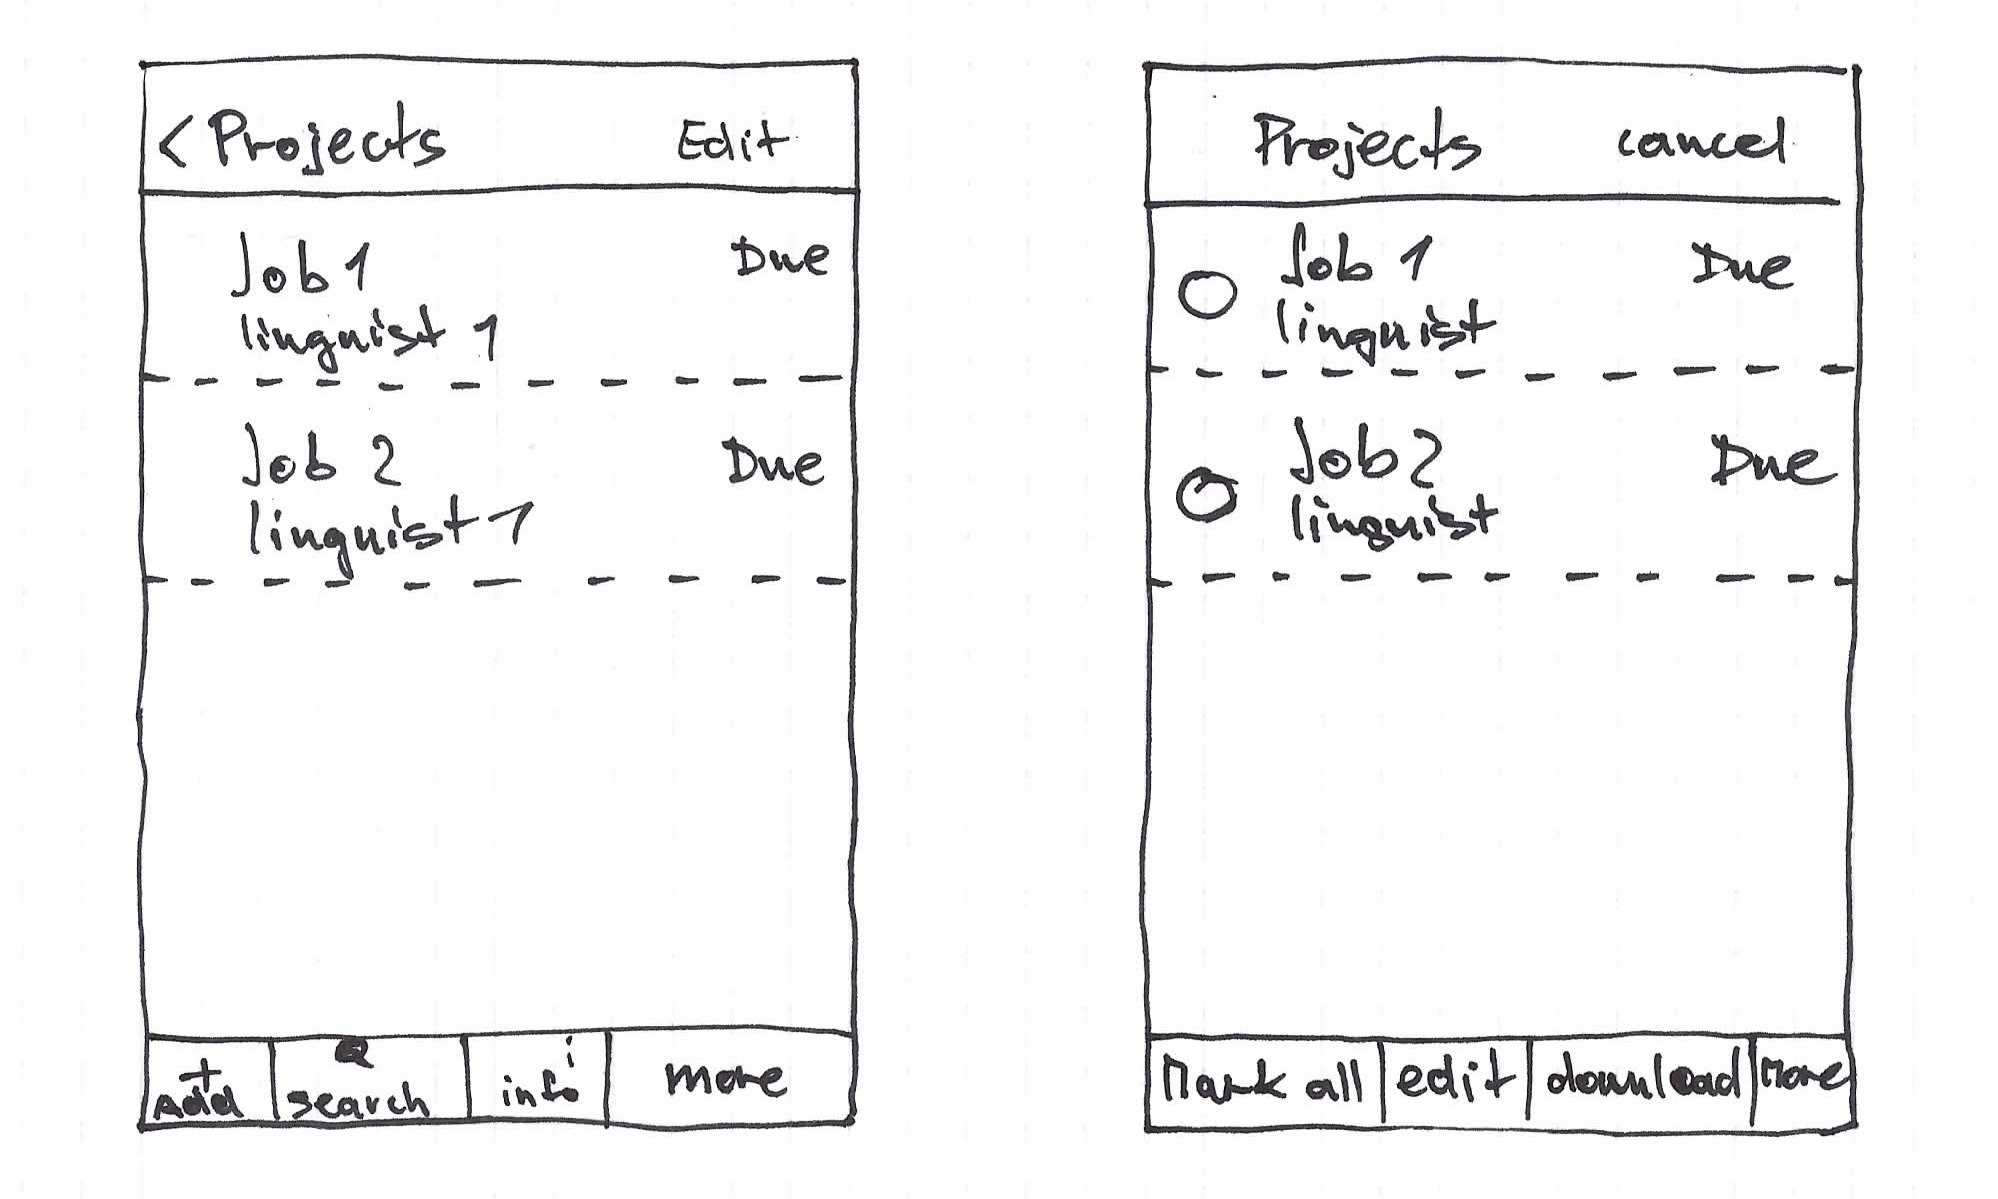
\includegraphics[width=0.8\textwidth]{pics/iosProjs2}
	\caption{Different way of listing jobs within a project on iOS. The second screen displays the state of the first after clicking on the 'edit' button.}
	\label{mock5}
\end{figure}



\subsection{Testing with users}

From the mockups I created a software prototype for Android. The prototype was created using Axure RP 8.0 \footnote{http://www.axure.com/} which is a software for creating different kinds of UI prototypes. There are widget libraries available, which contain ready-to-use Android and iOS UI elements. Figure \ref{fig:proto} show selected prototype screenshots.

To verify the created prototype, I conducted two informal tests with users. Axure provides Axure Share service to share projects, with and Android app \footnote{https://play.google.com/store/apps/details?id=com.axure.axshare} available on the Google Play Store, but this app proved not to be suitable for testing because it does not scale the UI well. Instead, I took advantage of Axure's ability to export created project as HTML which can be viewed directly on the device, for which I used the Kiosk Browser \footnote{https://play.google.com/store/apps/details?id=it.automated.android.browser.kiosk} app which allows to display content full-screen. 

To help keep the users relaxed, I explained the purpose of the application we were about to test and that we were testing only an initial prototype to catch its flaws, and not testing their abilities of working with Android.

The users were given a list of tasks corresponding to a possible walkthrough of the app. The text is following: 

You are a Memsource Cloud user and your role is project manager. Log in using the username ``user'' and password ``pass''. View translation jobs in Project 1 and download job whose name is ``Job name'' onto your device. Then create a new job from the ``document.docx'' which is available on Google drive. For the job, select English and German as target languages, due date as 2nd January 2016, 11:00 am and enter linguist name. You need the file be imported with comments and hidden text. Then, create a new project as new project name, enter ``test project'', select ``client 3'' as the client and select arbitrary parameters for the other options.

The informal testing was conducted in the company offices with two members of Memsource support team who both were owner of a mobile phone running Android. Test was conducted using LG Nexus 5 with the prototype running in the aforementioned Kiosk Browser. The downside of this setup was that the back button of the prototype was not available and in one instance (before adding a new project), this required intervention into the test process and consequent finding that a back button should be added to the navigation bar. Also, the generated html prototype seemed to have issues with entering text into textfields---they were accessible only after a long press instead of a simple tap. I have not found the root cause of this and needed to inform users of this issue before starting the test.

\begin{figure}[]
	\centering
	\begin{minipage}{.5\textwidth}
		\centering
		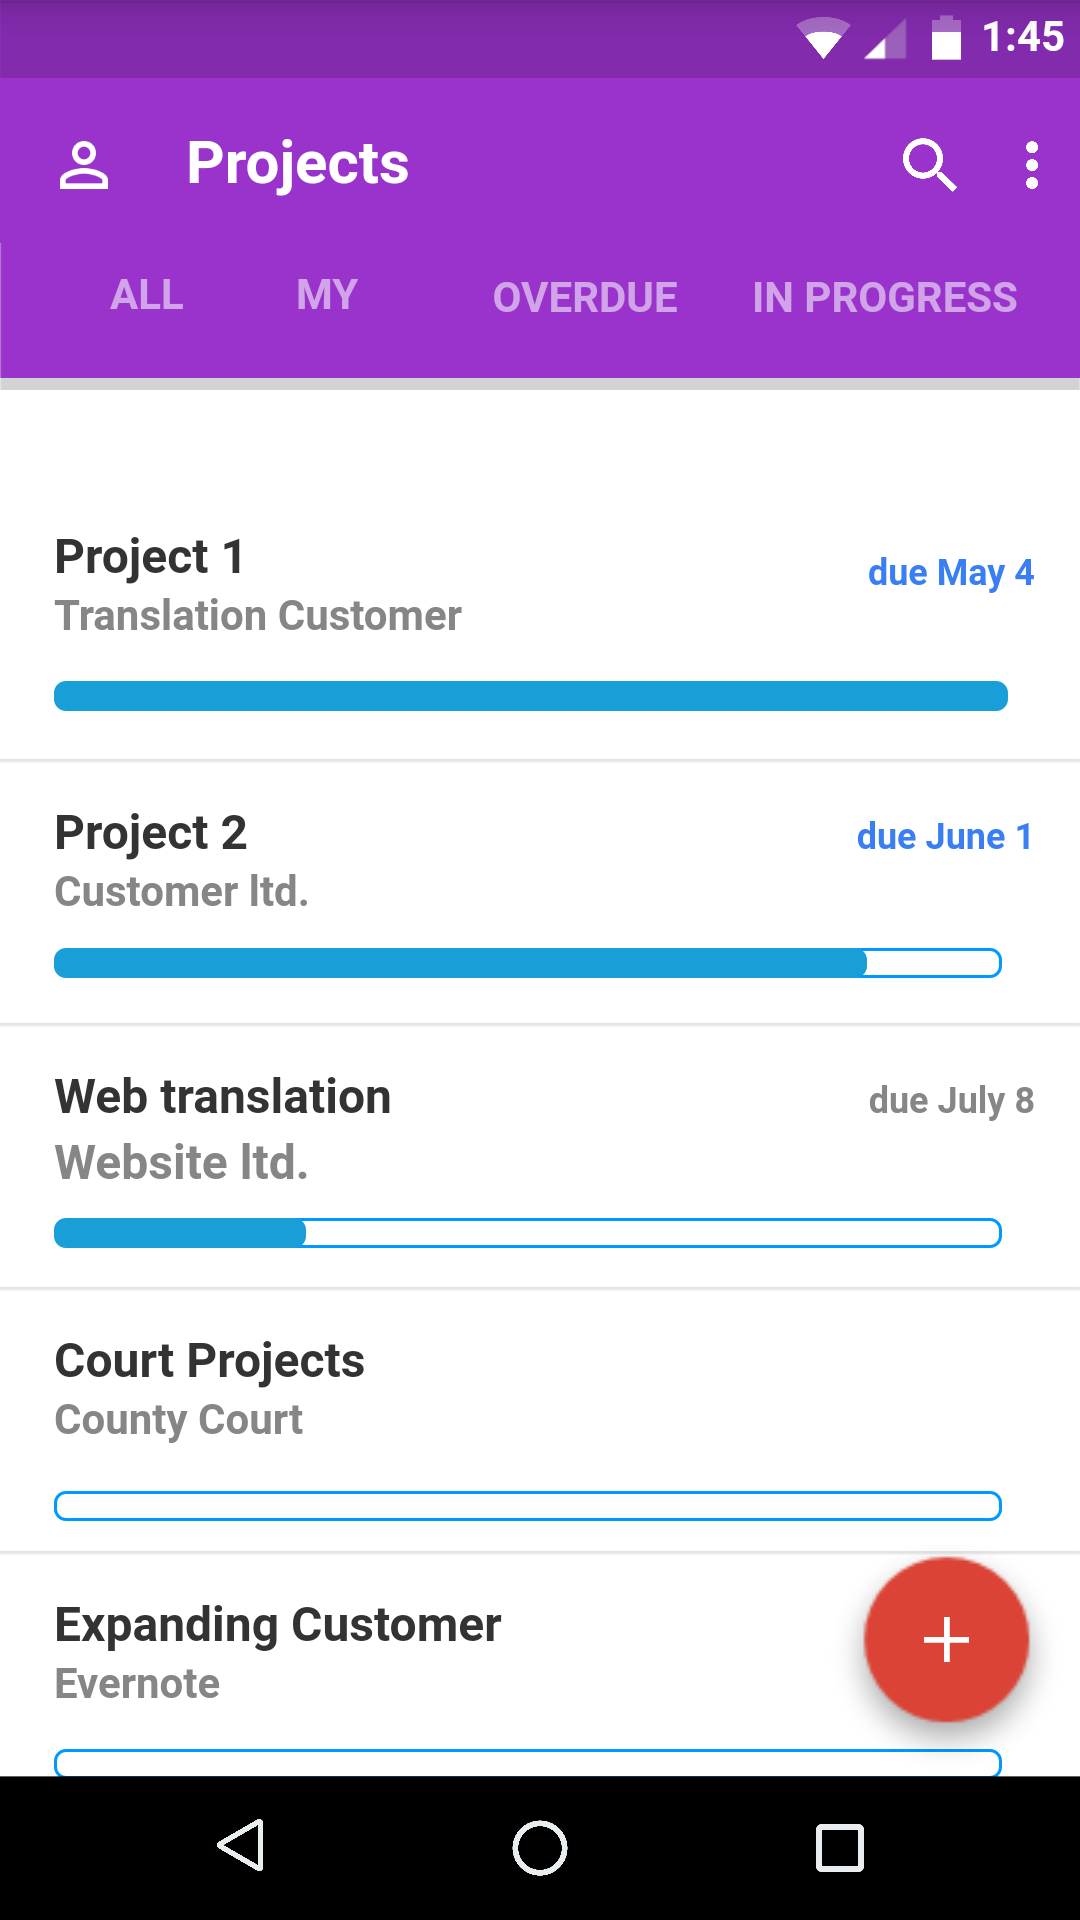
\includegraphics[width=.74\linewidth]{pics/protoProjects}

	\end{minipage}%
	\begin{minipage}{.5\textwidth}
		\centering
		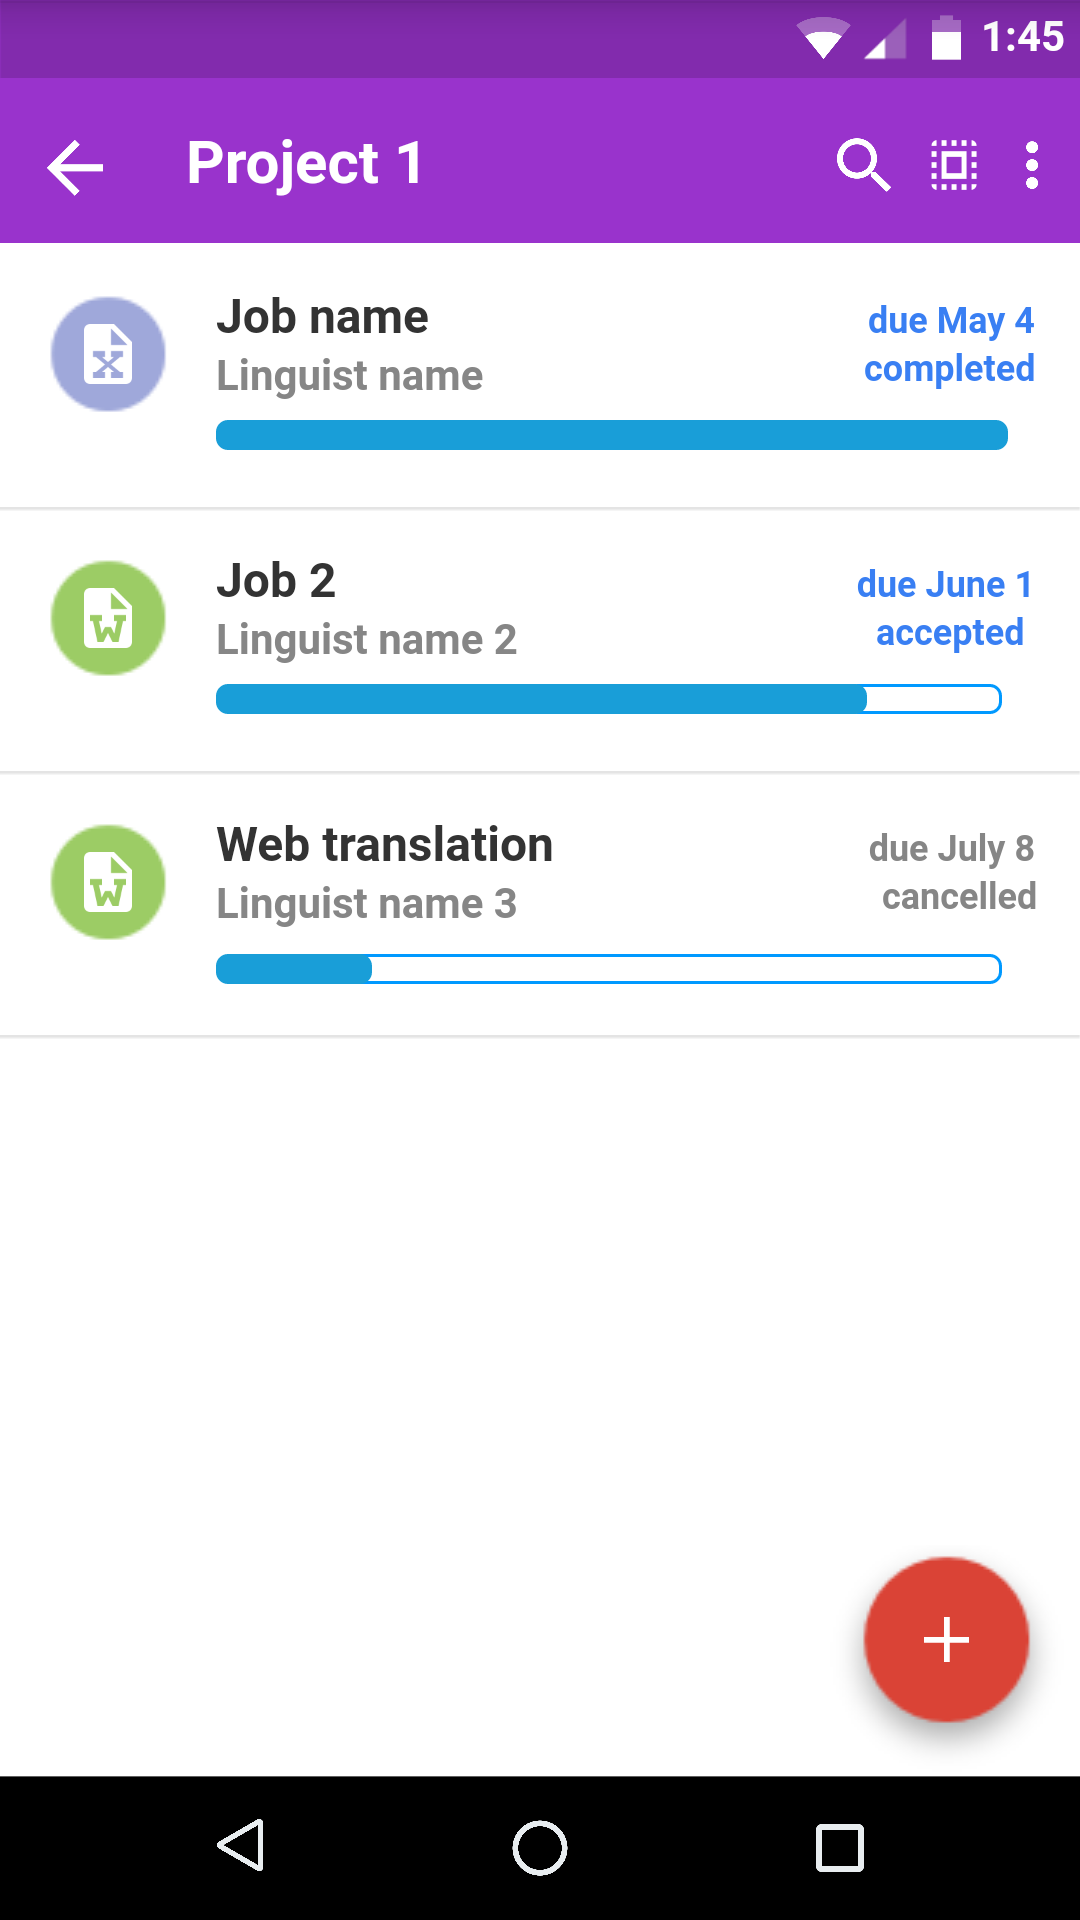
\includegraphics[width=.74\linewidth]{pics/protoProject1}
		
	\end{minipage}
	\caption{Listing projects (left) and jobs in a project (right).}
		\label{fig:proto}
\end{figure}


\subsection{Test results}

The test was completed by both users. However, during the test, two mistakes present in the UI were reported (problem with import options and adding new project). Both users complained about unintuitive icons, which was especially true of the white cloud icons in the upper right corner of the screen. After filling in all information for a new project, one user asked if that was the icon they were supposed to tap.

For the second iteration of testing, I used an improved prototype which fixed the flaws we found in the first iteration. Also, I stopped using the kiosk app and opted for the Axure Share Android app after fixing the scaling issue. The second test was successful and users reported they were satisfied. One tended to play with the prototype beyond the extend of what it was made for and complained some buttons were not functional. I do not consider that a problem, since this was mainly a horizontal prototype with only a particular interaction path implemented.



\section{Application Architecture}

In this section I describe the process of designing the inner workings of the application with respect to the fact that React Native was chosen as the library for implementing the application. This first involves finding a solution for app's state management which may fundamentally influence the architecture.


React Native allows to create user interfaces from the fundamental building blocks of the platform it runs on (\texttt{View} on Android and \texttt{UIView} on iOS) and it also provides means for communicating between the Javascript and native layers. What remains to be chosen is a library that will be used for storing the application state - ie. all of the data fetched from the Memsource API and displayed in the app such as project data, app user information and other. There are several libraries that help solve the problem. The most popular at the time of writing is called Redux \cite{stateOfJS}.

\subsection{Redux}

Redux is built around several core principles:
The entire app state is stored in a single object called the store \cite{redux:store}. The state can be modified by actions which are plain JavaScript objects describing the name and payload of the action \cite{redux:store}. Actions are dispatched to reducers. Reducer is a pure function that takes two arguments: previous state and action, and returns the new state.

Pure function \index{pure function} is a function that always returns the same result given the same parameters and produces no side effects. It is important that the reducer calculates the next state and returns it, without modifying the previous one.
As the application grows, the root reducer function is split into more reducer functions responsible for reducing different subparts of the state. Designing the shape of the state object is therefore key part of using Redux in any application.

Redux requires that the state is not modified in the reducer, which works well with the use of persistent immutable data structures \cite{redux:intro} (PIDS). The most popular implementation of PIDS in JavaScript is Immutable.js. Immutable.js offers data structures that present an mutable interface (such as add() method for an array) but instead of mutating the original object, a new object is returned, so using the reference equality operator will return false.

When changing an object in PIDS, the new object is essentially a copy of the previous one but as much content as possible is recycled from the previous object. Other objects that pointed on the old object need to be copied as well, but objects that do not need to be copied stay unchanged. Implementations of PIDs use Trie data structure to represent common data structures such as arrays using a tree. This is shown in the following figure todo. 

Lastly, Redux provides the redux-react package which allows the React components to "connect" themselves to relevant parts of the state tree and receive the data from them through props.


\subsection{MobX}

MobX is another state management library with growing popularity that has React bindings. MobX uses observable data structures that, as opposed to Redux, are mutable. Its key philosophy is that "Anything that can be derived from the application state, should be derived." \cite{mobx:intro}. Compared to Redux, MobX requires writing less code and while its internals are much more complex because of the change tracking, it offers synchronized state and views out of the box and its API surface is small.

With MobX, the first step is to declare the state and make the relevant parts of it observable. This is usually done in ES6 classes.
The next part is observing the changes in observable data. This is done through tracked functions. MobX tracks the observable data used during the execution of tracked functions and invokes them upon change in that data. 

One of the most important tracked function is \texttt{autorun}. If an observable data used in autorun changes, autorun is re-run. This is the function that is responsible for keeping the React views in sync with the observable state. MobX provides the mobx-react package which includes an \texttt{@observer} decorator which can be used for React component to make them react to changes in observable data, and the decorator makes use of \texttt{autorun} internally.
MobX also provides many other reactive utility functions for more fine-grained reactions. An example of how MobX can be used with React is shown in figure \ref{code:mobx} where a simple React component shows the number of seconds since the code was executed.


\lstinputlisting[label=code:mobx,caption=Using MobX with React]{./code/mobx.js}


After developing a small part of the application with Redux and also MobX, I chose to use MobX for storing the app state. The reasons for choosing MobX were its simplicity and proximity to object-oriented software design which I'm more experienced with. 
Using Redux requires writing boilerplate code to describe the actions and writing the reducers. Also, it is not always possible to dispatch actions that are plain objects - communication with Memsource API, for example, would require dispatching functions that would change the state after receiving data from the API. Working with hierarchies of objects also requires normalizing the application state, similar to how it is done in databases, with ids used as keys for retrieving a referenced object from other parts of the state tree. Apart from Redux itself, this then involves understanding several other libraries such as normalizr, redux-thunk (or other), reselect (optional) and Immutable.js (optional but much recommended).


With MobX, the app will consist of the views which are handled by React, domain objects, which are Javascript objects and some of their properties will be marked as observable or computed (ie. derived from other observables). The domain objects will be stored in domain stores. Stores are objects that instantiate new domain objects, delete the existing ones and provide other necessary functions with regard to domain objects. The last piece of the puzzle is handling communication with the Memsource API.

\section{Client-server Communication}

Communication with the Memsource API will be facilitated through an ApiCaller object whose simplified class diagram is shown in figure \ref{ApiCaller}. The documentation of Memsource APIs is publicly available at the \href{http://wiki.memsource.com/wiki/Memsource_API#API_Reference}{''Memsource wiki''}.

\begin{figure}[H]
	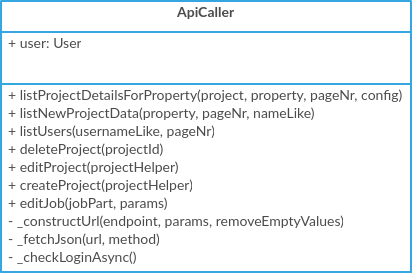
\includegraphics[width=0.6\textwidth]{pics/ApiCaller}
	\caption{ApiCaller class}
	\label{ApiCaller}
\end{figure}


ApiCaller will expose methods that offer CRUD operations over various resources such as project or jobs. All of its methods will return a Promise object which returns the fetched data upon resolving. ApiCaller will be used mostly from the stores and other functions needing API access. The advantage of having an object that will hide the fetching logic inside is easy testability and maintenance - if fetching is done in one place, it is easy to mock and change the implementation if needed. ApiCaller also contains a reference the currently active user, so that it fetches data in the user's name.


\section{Domain Objects and Stores}\label{sec:stores}

There are several core domain objects the application needs to work with. These represent the corresponding entities in Memsource Cloud and will be fetched through the API. These objects are mostly simple data holders, with little logic included in them. 

Domain objects will be stored in stores. Every type of object will have its own store that takes care of saving, editing and deleting the objects and may contain further logic needed to fulfill these tasks.
Figure \ref{Project} shows the Project class and figure \ref{projectStore} shows the store for projects. 

\begin{figure}[H]
	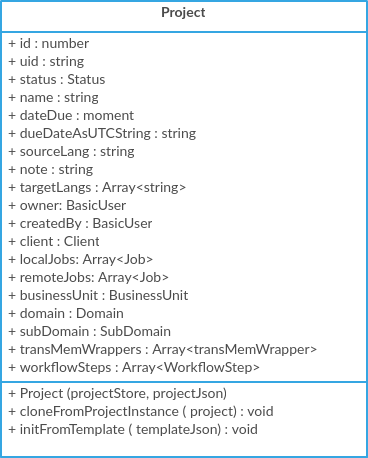
\includegraphics[width=0.6\textwidth]{pics/Project}
	\caption{Project class}
	\label{Project}
\end{figure}


\begin{figure}[H]
	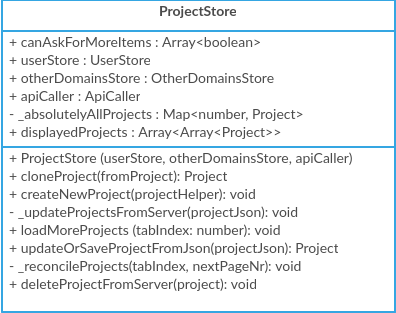
\includegraphics[width=0.6\textwidth]{pics/ProjectStore}
	\caption{ProjectStore class}
	\label{projectStore}
\end{figure}

For tasks such as creating projects or jobs, dedicated objects will be created, with their life span being limited by the sole task they need to fulfill.

\subsection{Representing Users}

Since the application has to support multiple users being logged in (with only one user being active at a time), we need objects for representing individual users as well as the collection of users who are logged in.

For this purpose, the User and UserStore classes are used. User instance contains data such as user name and id, and also user password, token, role and other. It is also the place where the user's search history is kept.

UserStore will contain an array of all users who are currently logged into the app, and a reference to the user which is currently active. Furthermore it will contain methods for creating new user instances and persisting the user information so that it is available upon application startup.


\subsection{Representing Jobs}




\subsection{Platform-specific Look and Feel}

React Native does not aim to provide developers with a way to run the same code on both platforms, instead it promotes the “learn once, write anywhere” paradigm and allows to create apps for both platforms while writing code using the same syntax.


Due to the nature of how both platforms are interacted with, we need to have an ability to make the user experience different per platform. As an example, take the Datepicker on Android versus the iOS Datepicker, or the Android navigation bar which often offers several actions (some with icons) versus iOS navigation bar which usually contains the title and no more than 2 actions. 
Actions that, on Android, would be included in the navbar, are often presented in a toolbar on the bottom of the screen on iOS, or hidden in an action sheet. Also note how Android works with long presses for item selection (for example in the Gmail app or the Downloads app), while this is usually done by an edit button in iOS navbar. The edit button then switches to an edit mode where user can perform their edits. If we want to follow these customs, this requires us to write separate code that would make the UI look and react to user actions differently on each platform, as well as custom code for the item selections and Android back button handling --- when in edit mode, the first back button tap disables the edit mode and only the second tap navigates to the previous screen.


React Native offers two ways how to go about platform-specific behavior. First is through the Platform module which gives information about the platform and its version. Another method is to use different file extensions (ie. \texttt{android.js} or \texttt{ios.js}) for components. The appropriate file will then be packed for the JavaScript bundle of each platform. Specifying what component to render by using different file extension is a powerful concept: typically a developer would use this approach for components that will serve the same purpose but need to look differently on each platform. Both files then have the same interface which abstracts away the inner differences. Such approach can be used in a number of components such as buttons, pickers or even a non-component code. I will take advantage of these features to improve user experience and to follow the design guidelines.


